\documentclass[../report.tex]{subfiles}
\begin{document}
\graphicspath{{img/}{../img/}}
This chapter describes the different design choices we have though about in developing the framework.

%To establish a vocabulary:
%    Situation - A physical situation eg. A person sitting down
%
%    Context - Context is knowing the situation and being able to react and be accordingly
%
%    Context information - Every information that aggregates a context

\section{Grand Architecture}
When looking at the blackboard and widget based methods, we have decided that we want to include a little of both.

We want to do a centralized system where clients can register a situation predicate. Our implementation, the OCon framework, will be event-based so when ever the state of a clients predicate changes, an event will be fired to notify the client. 

This combines the blackboards centralization and abstraction with the widgets time and space coupling. This will result in a solution where its transparent for the developer which sensor is actually given the input, like the blackboard, but also having the space and time coupling from the widget based method.

With this OCon will be an If-this-then-that solution where the client can use sensor input for control without the client developers having to put much though into using and managing sensors. This will be realized by three different components. A client, a central and a widget. 

\begin{figure}
\centering
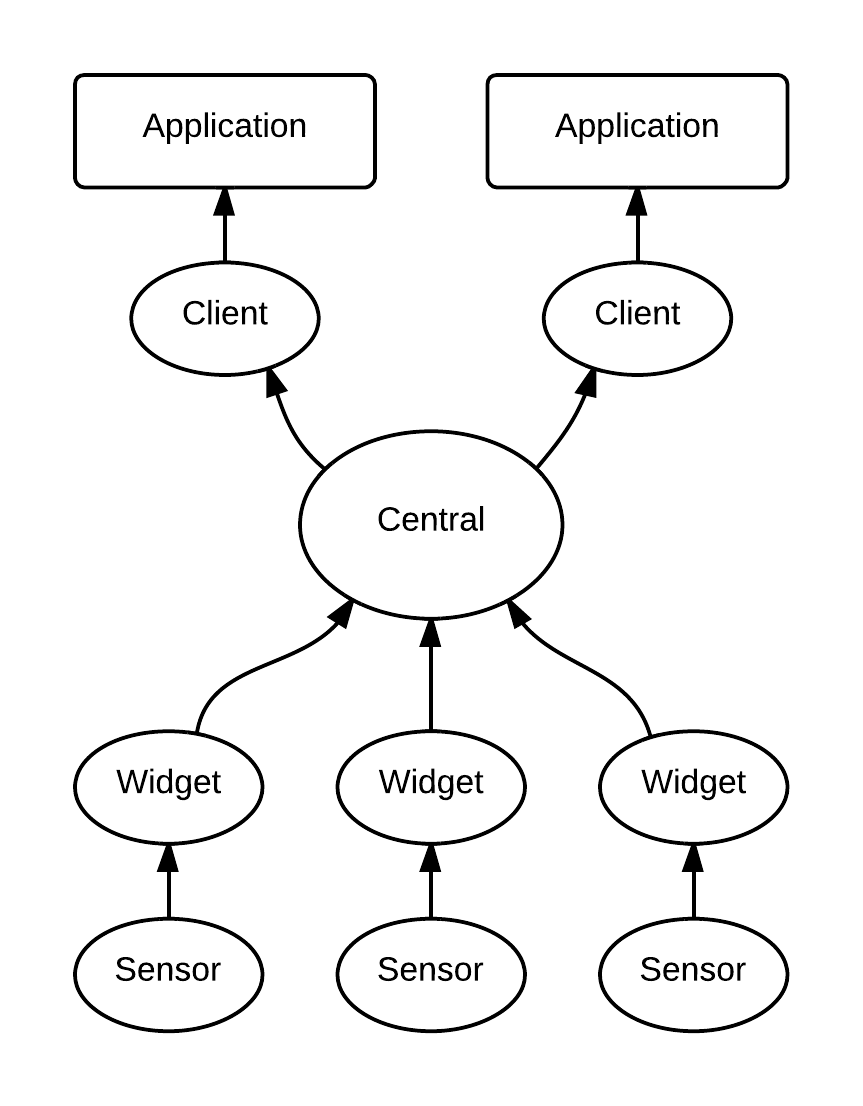
\includegraphics[width=200px]{grandarchitecture.png}
\caption{Grand architecture of OCon}
\label{fig:composite}
\end{figure}

\todo Please QA

\section{Encapsulation of Context-information}
Object-oriented encapsulation of context can be done in a variety of ways.

We have been looking at two different methods. Using a composite pattern and modelling with properties.

Using a composite pattern enforced relations between entities, entities being locations, persons, things or other real world objects.

Lets say we want to model a location with some rooms with some persons with different items or actions. Using the composite modelling we can have a location object containing room objects containing person objects containing item objects. We'll then have a relationship between the objects compositing the context being that a group of students is in room 3A04 at ITU all having phones in their pockets and all sitting down. This is a fairly complex, but a very extensible and flexible way to model situation (See fig \ref{fig:composite}). The downside to this method is that you can easily have an overflow of entities, and that it can be very complex and computation heavy to check against a predicate.

The other method we are considering is more simple. Having a set of entities that we wish to track, eg persons. All context information relating to a person will be properties to the object. So to use the previous example, a person entity would then have a location property, being ITU room 3A04, a phone property begin true and a sitting property being true. This model is more easy to make, but it limits the developer to know very precisely what information is needed and should be tracked. The previous model had the advantage of being very flexible allowing more complex relations and situations. 

Both methods have pros and cons being how dynamic they are, how easily they can be implemented, and what performance they will have and that will be the parameters we'll look at when implementing OCon 

\begin{figure}
\centering
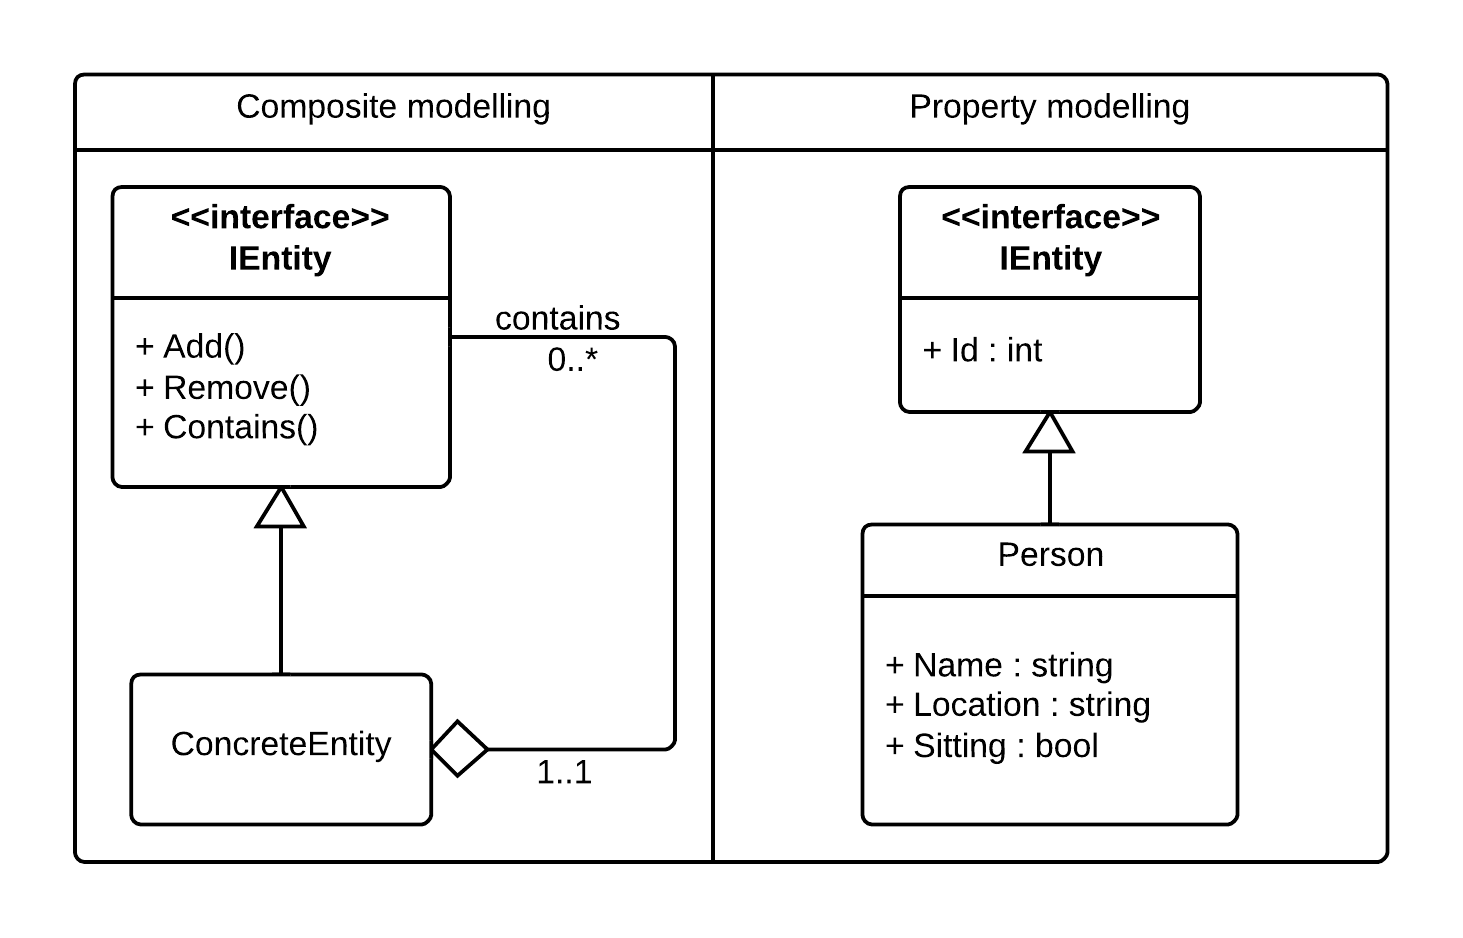
\includegraphics[width=200px]{composite.png}
\caption{Diagram illustrating composite modeling}
\label{fig:composite}
\end{figure}


\section{Central}

Then central is the central competent and will facilitate clients adding predicates for the central to track. When an entity change is received relevant to the predicate, the predicate will be checked and if its state changes, the owning client will be notified.

The definition of predicate is taken from the .NET platform. A predicate is a delegate returning a boolean. In this way .NET developers will be familiar with the meaning and definition of a predicate.

A important feature to be included with our central is the ability to be discovered by client and widgets. The central will be able to broadcast itself to the chosen distribution channel and to widget and client will then be able to discover and connect to the central. This feature will enforce a more dynamic usage and behaviour of OCon.

\todo Please QA
 

\section{Widget}

In OCon widgets will translate sensor input to entities along with facilitating the communication to the central.

This approach have been chosen to make the system easily distributed as a small, maybe embedded, component can facilitate as widget translating the sensors input to entities before sending them to the central.

This approach will also reduce network load as the widget will only send updates to the central when changes occur. This stands in contrast to sending all sensor input to the central and making it process the data itself which could be useful in some cases.

Latests would also put more computational pressure on the central making it hard to scale to larger systems.


\section{Client}

The client will be the entry point into OCon facilitating developers to add situations to the central and receive updates whenever an update to those situations occurred.

The client will be able to automaticly discover and use the central. 

\todo What do we do with this chapter?


\section{Communication}

Initially we decided that making the OCon distributed would be out scoped, but as the project progressed it was decided to bring it into scope. Clients and widgets will be distributed from the central. The reason for doing so is that our vision of having a centralized system distributing situation from sensors to clients is not very useful if not distributed.

For the OCon two different communication protocols need to be implemented.\\

\begin{itemize}
    \item A protocol for establishing link between peers
    \item A protocol for send text/json messages for subscriptions, subscription events and, sensor events \\
\end{itemize}

We do not wish to bind our users to any concrete communication protocols. Therefore the communication will be interfaces so a concrete implementation can be dependency injected into the OCon.
\end{document}